\section{Composite marginal likelihoods}
\label{sec:piecewise}

The previous section provided a method of moments estimator
which used (i) tensor decomposition to recover conditional moments,
and (ii) matrix inversion to recover the hidden marginals.
Now we aim to improve statistical efficiency by replacing (ii) with a likelihood-based objective.

% DONE: set the stage a bit more
Of course, optimizing the original marginal likelihood is subject to local optima.
We make two observations to arrive at a convex optimization problem.
The first insight is that we have used tensor decomposition to recover the conditional moments,
so effectively a subset of the parameters have been fixed.
However, this alone is not enough, for the full likelihood is still non-convex.
The second insight is that we can optimize a \emph{composite likelihood objective} \cite{lindsay88composite}
rather than the full objective.

%The method of moments approach to recover parameters for each clique
  %$\sC$ presented in the previous section is easy to understand and
  %analyze, but sensitive to noise. 
%In this section we propose an alternate solution, optimizing the 
  %likelihood for each clique, that is more robust to noise.
We show that under the same conditions as \algorithmref{directed}, the
  negative composite likelihood function is strictly convex and thus
  tractable to estimate exactly.
  %guaranteeing that
  %gradient-based optimization will converge to the unique global
  %optimum.

Consider a clique $\sC = \{h_{i_1}, \cdots h_{i_m}\} \in \sG$, with
  exclusive views $\sV = \{x_{v_1}, \cdots, x_{v_m}\}$. 
The expected composite likelihood over $\Sx{\sV}$ given parameters $\mH_\sC$
with respect to the true distribution $\sM_\sV$ can be written in tensor form:
  [DONE: likelihood is a function of parameters, not of data]
\begin{align*}
  \sL_\ml %(\Sx{\sV}) 
  &= \E[\log \Pr( \Sx \sV )] \\
  &= \E[\log \sum_{\Sh \sC} \Pr( \Sx \sV \given \Sh \sC )] \\
  &= \E[\log \mH_\sC(\mOpp{v_1}{i_1} [x_{v_1}], \cdots, \mOpp{v_m}{i_m} [x_{v_m}])] \\
  &= \E[\log \mH_\sC(\mOppAll[\Sx\sV])].
\end{align*}
The final form is an expectation over a log of linear function of $\mH_\sC$, which is concave in
$\mH_\sC$.  But unlike maximum likelihood in fully-observed settings,
we do not have a closed form solution, so we use EM to optimize.
Since the function is convex, EM converges to a global optimum.
\algorithmref{piecewise} summarizes our algorithm.

\begin{algorithm}
  \caption{\LearnClique (composite likelihood)}
  \label{algo:piecewise}
  \begin{algorithmic}
    % DONE: interface should match LearnClique from directed.tex  
    %\REQUIRE A graphical model $\sG$ satisfying \propertyref{bottleneck}, data $\sD$
    %\ENSURE Marginals $Z_\sC$ for every clique $\sC \in \sG$
    \REQUIRE Clique $\sC$ with exclusive views (\propertyref{exclusive-views}).
    \ENSURE Marginal distribution of the clique $Z_\sC$.
\STATE Identify exclusive views $x_\sV = \{x_{v_1}, \cdots, x_{v_m}\}$.
\STATE Return $\hat \mH_\sC = \arg\max_{\mH_\sC \in \Delta_{k^m-1}} \sum_{\vx \in \sD} \log \mH_\sC(\mOppAll[\Sx \sV])$.
%      Run expectation-maximization to convergence on the piecewise likelihood \eqref{eqn:piecewise}, over data $\{\vec x_\sC : x \in \sD\}$
  \end{algorithmic}
\end{algorithm}

\subsection{Statistical efficiency}

We have proposed two methods for estimating the hidden marginals $Z_\sC$ given
the conditional moments $\mOppAll$: one based on computing a simple pseudoinverse,
and the other based on composite likelihood.
We use the notation $\hat Z^\mom_\sC$ to denote the pseudoinverse
  estimator and $\hat Z^\ml_\sC$ to denote the composite likelihood
  estimator.

The Cramer-Rao lower bound tells us that maximum likelihood yields
the statistically the most efficient composite estimator for $Z_\sC$
given access to only samples of $\Sx\sV$.\footnote{Of course, we could improve statistical efficiency
by maximizing the likelihood of all of $\vx$, but that would again lead to non-convex optimization problems.}
But can we quantify the \emph{relative efficiency} of the pseudoinverse estimator
compared to the composite likelihood estimator?
Let us first compute the asymptotic variance of the latter.

\begin{lemma}[Asymptotic variance of the composite likelihood estimator for $Z_\sC$]
  \label{lem:pw-variance}
  The asymptotic variance of $\hat Z^\ml_{\sC}$ based on composite likelihood is
  \begin{align*}
    \Sigma^{\ml} &= \mOppAlli \dM_\sV \Sigma_\sV \dM_\sV \mOppAllit.
  \end{align*}
\end{lemma}
\begin{proof}
  The result follows by direct application of the delta-method
  \cite{vaart98asymptotic} to the negative-likelihood objective. Refer
  \appendixref{pw-variance-proof} for a complete derivation.
\end{proof}

%%%%%%%%%%%%%%%%%%%%%%%%%%%%%%

The following lemma shows that the gap between the two estimators can be quite substantial,
and scales with the dimension $d$: % \todo{make sure this is true}:
\begin{corollary}
The pseudoinverse estimator is strictly less efficient
than the composite likelihood estimator in that $e^\mom \eqdef \Tr(\Sigmamli \Sigmamom) < 1$.
\end{corollary}
\begin{proof}
  From \lemmaref{mom-variance}, we have the asymptotic variance of the method of moments estimator, $\hat Z_\sC^{\mom}$ is,
  \begin{align*}
    \Sigma^{\mom} &= \mOppAlli \Sigma_\sV \mOppAllit,
  \end{align*}

  By \lemmaref{pw-variance}, we have the asymptotic variance of the piecewise likelihood estimator, $\hat Z_\sC^{\ml}$ is,
  \begin{align*}
    \Sigma^{\ml} &= \mOppAlli \dM_\sV \Sigma_\sV \dM_\sV \mOppAllit.
  \end{align*}

  Note that $\Tr(\dM_\sV) = 1$ as it represents the marginal
  distribution of $\sV$; thus, $\Sigma^{(\mom)} \succ \Sigma^{(\ml)}
  \succ 0$.  Finally the asymptotic efficiency of the method of moments
  estimator is, 
  \begin{align*}
    e^\mom &= \Tr( \Sigma^{\ml}\Sigma^{\mom -1} )  \\
           &= \Tr( \dM_\sV \Sigma_\sV \dM_\sV \Sigma_\sV^{-1} ) .
  \end{align*}
\end{proof}

\paragraph{Intuitions}
%It is well known that the method of moments estimator is less
  %statistically efficient than the maximum likelihood estimator. 
To get a sense for how large the gap is, consider an example in which
$M_\sV$ is close to the uniform distribution, i.e. $\dM_\sV
  \approxeq \frac{1}{d} I$. 
Then the efficiency of the $e^\mom \approxeq \Tr(\frac{1}{d^2} I) = \frac{1}{d}$.
In other words, the gap in variance between the method of moments
  estimator and maximum likelihood grows linearly with the number of observations $d$.

% (ARUN): Possibly cut this whole part.
\figureref{cl-hmm} compares the parameter recovery error of the
  pseudoinverse estimator and the composite likelihood estimator for
  a hidden Markov model with 2 hidden states ($k=2$) and 3 emissions
  ($d=3$).
Empirically, we observe that using the composite likelihood estimator
  was more stable and leads to better results.

% Visualize
% To visualize this phenomenon, note that the pseudoinverse estimator can be written
% as $\hat Z_\sC = \argmin_{Z_\sC} \|Z_\sC \mOppAll - M_\sV \|_F^2$.
% \figureref{piecewise-objective} plots the compares the objective values for
% different choices of the $\pi$ parameter in a hidden Markov model
% (\figureref{examples-hmm}) with 2 states ($k=2$) and $d=10$ dimensions.
% Note that the negative log-likelihood objective is more
% strongly convex than the pseudoinverse objective.
% \todo{this is perhaps misleading, you could get the plot with the same with $100000000000 x^2$ and $x^2$.
% Let's talk about this.  If can't fix, remove.
% }

\begin{figure}
  \centering
  %  \subfigure[Comparing the piecewise objective with the moment-matching objective] {
  %    \label{fig:piecewise-objective}
  %    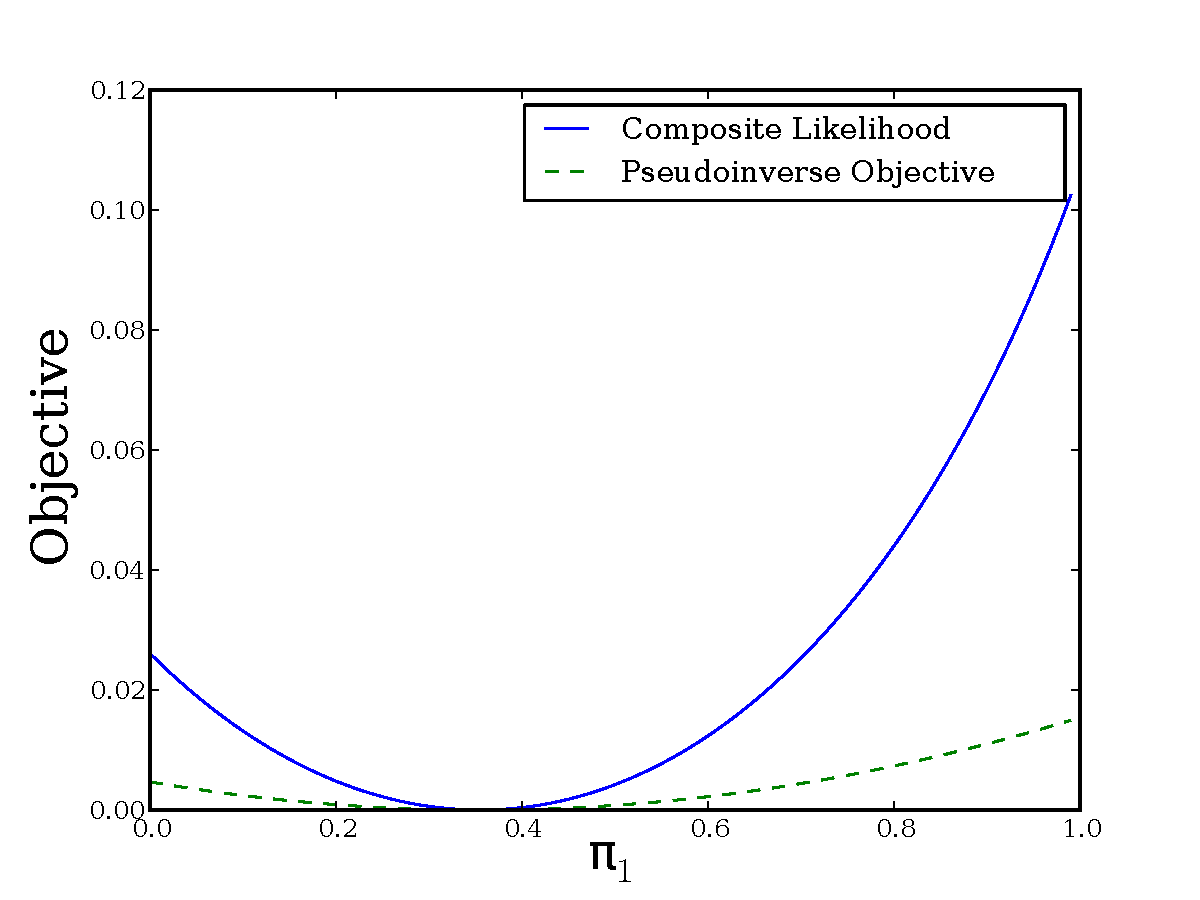
\includegraphics[width=0.45\columnwidth]{figures/piecewise-objective.pdf}
  %  }
%  \subfigure[Directed grid model] {
%    \label{fig:examples-grid}
%    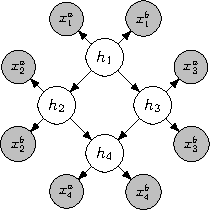
\includegraphics{figures/grid.pdf}
%  }
%  \subfigure[] {
  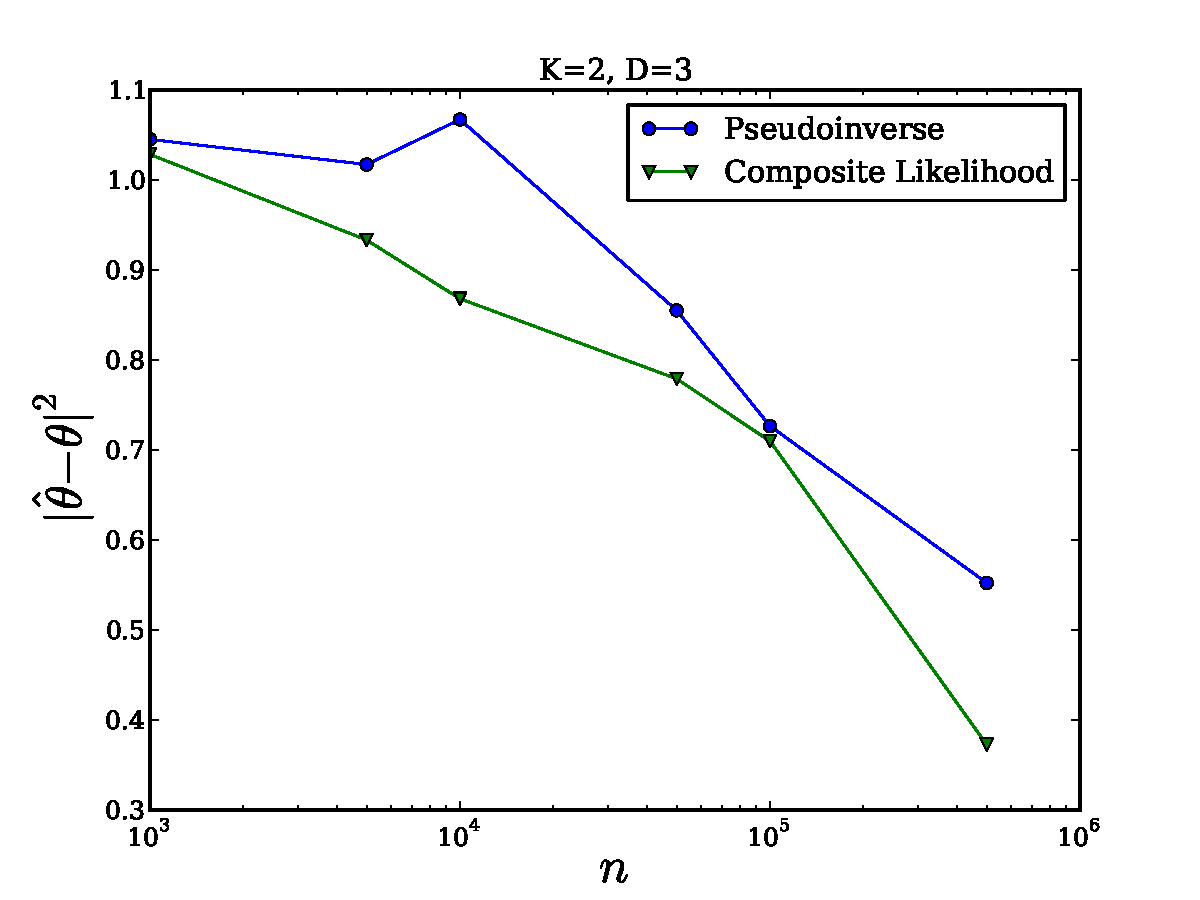
\includegraphics[width=\columnwidth]{figures/hmm-2-3.pdf}
    \label{fig:cl-hmm}
%  }
  \caption{Empirical performance when recovering parameters for a Hidden Markov Model with $k=2$ states and $d=3$ emissions}
\end{figure}
